This document summarises the major contributions of Saulius Lukauskas
to the development of \means{} package.
This document has been written as a succinct supplement to the group report, and therefore it contains numerous back-references to sections of the larger document.

\section{Introduction}

\section{Contributions}
\subsection{Software Development Process}
\todo{Quote science code manifesto}
In the modern day where computers are becoming the driving force of innovation and progress the whole world is facing the need to either adjust to this computerisation or risk to be left behind by others.
Naturally, scientific software is becoming critically important for scientific communities in every major field of science. This importance raises the demand for scientists who are also proficient in computer programming. However, while knowledge of computer programming is deemed critical, the necessity to study software engineering is still being debated. 

The common argument for the lack of need to study software engineering, claims that people often care only about the end result, and not how it was obtained or how easy-to-read code is.
To me this claim seems to be ironic as the same argument can be used to describe the main reason why the software-engineering methodologies emerged in the first place. 
For instance, two of the main principles of the \emph{agile} methodology\cite{_manifesto_????} claim treat the ``working software as the primary measure of success" and claim that ``simplicity -- the art of maximising of work \emph{not} done -- is essential"\cite{paulk_agile_2002}. 
In fact \emph{agile} methodology is often viewed as an alternative to the approaches that aim to create this idealistic, properly structured and well-documented software, such as the traditional \emph{waterfall} model.

It was my personal goal, and I believe my biggest contribution, to share my experience in software engineering in order to incorporate the \emph{agile} methodology into our development cycle. 
In this project I aimed to introduce my peers to concepts that might have not been known to them previously as well as to try to validate their value by showing the value they bring. 
This section lists a couple of the modern software development practices we aimed to employ, and provides a short description of how they contributed to the success of \means{} project.

Whenever I introduced a concept to the peers, regardless if they have heard it before or not, I also tried to push it to further to the limits, so the biggest advantage can be seen. 
For instance, not only we were using \verb"git"\cite{git} for our version control, but we were also using appropriate branching workflow. 
This allowed each one of us to work on separate things in isolation, and ensured one's changes will not break the other's work. 
In turn this provided the courage for us to be able to experiment with the code more, knowing these experiments will not impact others.
Without this courage, performance improvements described in the group report's section \autoref*{GR:performance} may have never been made.

Another factor that contributed to the ability to change the key parts of the system without the fear of breaking something was the early incorporation of automated tests to the system. 
This created a way to validate the correctness of our software quickly.
Similarly, it allowed us to pin-point the location of a failure quickly, minutes after it occurred.
These automated tests allowed us to spend less time testing our software, but trust it more.
In turn, this had a positive effect on our confidence in the validity of the observations made (as described in the \autoref*{GR:results} of group report). Our approach to software testing is summarised in the main report's \autoref*{GR:sec:testing}.

To help ourselves \emph{increase the amount of work not done}, we set up a continuous integration server.
This server, implemented by the \emph{Jenkins CI} platform\cite{_jenkins_????}, has responsibly been running every single test we have after every single push to the central code repository we made. At the moment of writing, the server has run 507 of these tests.
We assumed that if the code does not work on \emph{Jenkins}, as we called it, it does not work at all, regardless of whether the code works on the author's machine or not. 
Such code could then be retracted, fixed and pushed again to the main repository, at which point it will be tested again. 
This central server allowed us to reduce the number of times we have to deal with issues occurring due to simple human error, such as files forgotten to be added to the central repository, or tests not run before a commit to the code repository.

Similarly, \emph{Jenkins} enabled us to run code in different environments. For instance, we kept all the libraries updated to the latest version in one of the environments we ran the code on. 
It was because of this special environment that we spotted an incompatibility with the latest version of \verb"Assimulo"\cite{andersson_christian_assimulo:_????} -- the package providing ODE solver implementations in \py{} -- minutes after that version became public. We were then able to prove that this incompatibility was a problem with the \verb"Assimulo" package, not ours. 
We then worked together with Cristian Andersson (one of the developers of \verb"Assimulo") to it get fixed and new version of the package released.
In the sense, this continuous integration environment has contributed to two projects -- \verb"Assimulo" and \means{} -- as if not for it, said bug in the library might still be present today.

Finally, I explained in detail the advanced concepts of Object-Oriented Programming, such as inheritance, encapsulation, static methods to my peers so they could be applied in our project.
I attempted to show how these concepts make the code both easier to maintain, and easier to write in the first place, hopefully allowing the peers to transfer these skills to their other projects as well.
In the end, I believe we have succeeded at creating a highly modular codebase, which should be easy to maintain in the future. The summary of our code base is available in the \autoref*{GR:sec:package} of the group report, as well as in the documentation, described in the appendix \autoref*{GR:sec:documentation} of group report.

Besides the programming-related best practices of software engineering, we also implemented certain project management aspects suggested by \emph{agile} methodologies. 
For instance, we structured our work into weekly iterations. We were planning the things we need to do for the week, and reviewing the things we done at the end of it. 
We have structured our iterations to end just before the weekly meetings with supervisors, so we could also immediately get the feedback.
This allowed to keep the project on a clear track, going the right way and within the scope required.

In the end, I believe that the software-engineering approaches I described above acted both as an educational exercise and a way to be more efficient, when it comes to software development.
I strongly believe that without them, we would not have been able to progress as much with the project as we did.
I also hope that the anecdotal evidence listed above may serve as a proof of utility of software engineering approaches, however small, and maybe act as an argument in favour of it as well.

\subsection{Significant Code Contributions}

In the previous section I have talked about the software development process in general and my contributions to it. 
Below I list my most noteworthy contributions to the source code of \means{} as well as justify some of the design decisions we made.

\subsubsection{Implementation of Simulation Routines}

It is no secret, that we did not start this project from scratch.
The previous year's MSc students have already contributed a large quantity of \py{} code that provided some basic functionality of \means{}. In this project, we aimed to attempt to simplify the said functionality and therefore it easier to use and maintain (see \autoref*{GR:sec:aims_of_the_project} in the group report).
To do this, we reviewed the code and marked the parts of it that we felt could have been replaced with something else. 
We then approached these parts, one by one, and refactored them in isolation, aiming not to break the remaining parts of the system.

One of the first things I, myself, worked on in this project was an attempt to simplify the simulation mechanism implemented the previous year's version of the code. In a nutshell, this original mechanis split the process into three parts: first the \python{} code was transcribed of into C code that interacts with the \verb"CVODE" library\cite{hindmarsh_sundials_2005}, which then was then compiled, and later on run directly from \py{}.

We felt that his rather \emph{ad-hoc} process of transcribing \py{} to C seemed to be error prone and unnatural in general. 
Similarly, \py{} code was interacting with the compiled C library in a platform-specific and multiprocess-incompatible way, reducing the portability and possible uses of the code. In our view, these two factors justified the need to replace this system.

We found \verb"Assimulo" -- a package already mentioned once before in this report -- to be a suitable replacement for the wrappers around \verb"CVODE" that would allow us to easily extend the functionality as well. 
I have prototyped and implemented the code change replacing the mechanism described above with a cleaner mechanism offered by the \verb"Assimulo" package. This also allowed us to add the sensitivity analysis support to the \means{} package as well as the ability to run the simulations using a different \gls{ode} solver.
This new interface is further described in detail in \autoref*{GR:sec:package_structure:simulation} and demonstrated in\autoref*{GR:sec:simulation} of the main report.

While \verb"Assimulo" handled much of the heavy-lifting when it comes to solving \glspl{ode}, we still needed to increase the performance of the numeric evaluations of the symbolic expressions. 
Previously this was a non-issue as these expressions were transcribed to C in the first step of the old process. 
Luckily, \verb"sympy" -- the python package for symbolic mathematics --provides a collection of methods of evaluating these expressions efficiently. QG and I have investigated these methods.
We benchmarked the \verb"lambdify" method, that turns the numeric expression into a \verb"lambda" function and the use of  \verb"autowrap" module which compiles the numeric expressions to C.
We did not test the third option -- Theano\cite{bergstra_theano:_2010} -- available in the latest version of \verb"sympy", because the college environment did not support it at that time\footnote{We eventually updated the college environment to run the latest version of the package, however we did not get back to this benchmark due to the time constraints.}.

\begin{table}
    \centering
    \begin{tabular}{l|l}
    Method & Runtime \\
    \hline
    Default & 628 microseconds \\
    \verb"lambdify" & 10.7 microseconds \\
    \verb"autowrap" & 2.89 microseconds \\
    Theano & not measured \\
    \end{tabular}
    \caption{Results of the three out of four numeric evaluation methods available in {\tt sympy}. 
    The results were recorded using the {\tt \%timeit} 
    function provided by IPython\cite{perez_ipython:_2007} interactive environment. 
    This function performs as many evaluations of the code it can fit in 2 seconds and returns the best runtime of all the repetitions.
    The evaluations were performed on the two right-hand-side equations resulting from approximating the dimerisation model up to the moment order of two.
    It is clear from the data that{\tt autowrap} method is a clear winner. 
    Theano performance was not tested as it was not supported in the college environment at the time we performed this test.}
    \label{tab:numeric-runtimes}
\end{table}

The benchmarking results from the experiment are summarised in \autoref{tab:numeric-runtimes}. 
We can see that \verb"autowrap" is clear winner in the benchmark and therefore was chosen to be implemented in our package.
This has proven to be an efficient-enough solution for most of the day-to-day needs, becoming an issue only for high-maximal order moment closures, where the number of expressions to evaluate is large.

In the future, however, it would be interesting to benchmark the Theano performance, whose inhering GPU support could speed up the evaluations even more.
In particularly, I believe it would help to reduce the exponential slope of runtime arising from the exponential increase of the number of equations as the maximal moment order is increased (see \autoref{GR:fig:solver-runtimes} in the group report) to make the simulations feasible for even higher orders. 

\subsubsection{Implementation of Inference Routines}

Similarly to the simulation methods described above, I have also worked on restructuring the parameter inference to make it easier to use from interactive environment. 
Namely we aimed to unify the interfaces to parameter distance methods regardless of the distance function used, and allow the user to specify the requirements succinctly.
I believe that both of these requirements were met, and the new interface for parameter inference is demonstrated in \autoref*{GR:sec:parameter_inference} of the group report.

Additionally, the unification of the parameter inference interfaces enabled our users to design their own distance functions, as demonstrated in \autoref*{GR:sec:distance_measures} of the group report.
Finally, I have worked with SF on the additional plotting functionality for the parameter inference results, such as the contour plot of the distance landscape, illustrated in 
\autoref*{GR:sec:investigating_distance_landscape} of the group report.

\subsubsection{Pipeline Support}

In the final days of this project, when we were generating the figures for the results section in the group report (\autoref{GR:results}), we realised that the scale of these figures was becoming hard to manage. 
At this point each one of us has had already written a couple of lines of code to perform the \acrlong{mea}, and store a result, a loop of some sort that would run simulation or parameter inference procedures on this result, and a way to store these results to a file. 
Errors with these methods were starting to crop up, for instance maybe somebody forgot to handle the solver errors appropriately and the task was supposed to run overnight failed, or maybe the task succeeded to run, but results were not stored in the correct format, rendering them unreadable, etc.
Similarly, we were unlikely to be able to share the results with each other and reuse, as they were all stored in different formats.
Something had to be done to reduce the number of these issues.

I proposed to use \verb"luigi"\cite{_luigi_????} -- a \python{} library developed by the engineers in \emph{Spotify} -- to provide an unified framework for the common tasks we had to do. 
The \verb"luigi" allows to break down complicated tasks into a set of smaller ones and specify the interdependencies between them.
The system could then find the most efficient way to perform these  tasks, often in parallel, so all of the tasks are executed before their parents in the dependancy tree. 
This is exactly the same concept as the one implemented by \emph{GNU Make}\cite{gnumake}, for those who are familiar with it. Unlike \emph{Make}, however, \verb"luigi" package is able to handle parametric tasks better, and is written in \py{}, therefore able to integrate with our codebase seamlessly.

I have particularly worked on writing the general wrappers around the means code in the \verb"luigi" framework. 
For instance, I implemented the \verb"MEATask" objects that would take a model, \gls{maxord}, closure method as a parameter and return the resulting set of equations corresponding to \gls{mea} approximation requested. 
This task was then the only dependancy of the \verb"TrajectoryTask", which used the set of equations generated earlier to simulate the behaviour of the system. 
In order to generate figures such as the contour plots shown in \todo{link here to next section}, a new task for the figure would be created, that would require a set of these \verb"TrajectoryTask"s to be performed. 

In turn, this allowed us to specify each figure in the report in a very high level language specifying only the dependancies of the task and the ways to combine them to get the result, without worrying on how to obtain these dependencies in the first place.

\begin{figure}
    \centering
     \begin{subfigure}[t]{0.3\textwidth}
        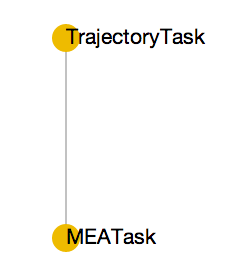
\includegraphics[width=\textwidth]{images/TrajectoryTask.png}
        \caption{Dependancies of {\tt TrajectoryTask}}
        \label{fig:pipes_example:TrajectoryTask}
    \end{subfigure}
    ~
    \begin{subfigure}[t]{\textwidth}
        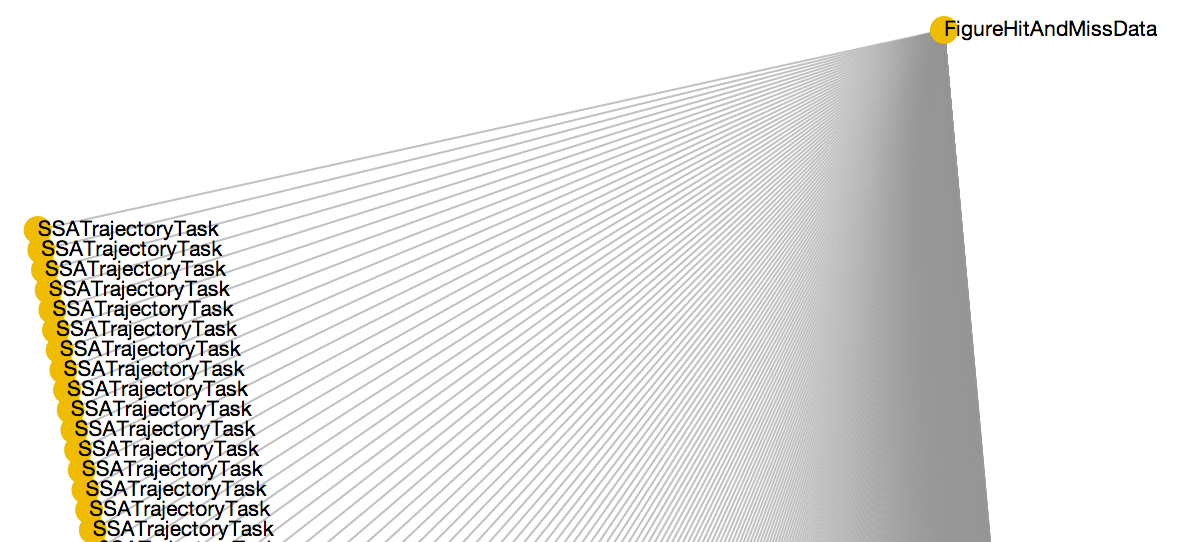
\includegraphics[width=\textwidth]{images/FigureHitAndMissData}
        \caption{Partial dependancies of {\tt FigureHitAndMissData}}
        \label{fig:pipes_example:FigureHitAndMissData}
    \end{subfigure}
    ~
    \begin{subfigure}[t]{\textwidth}
        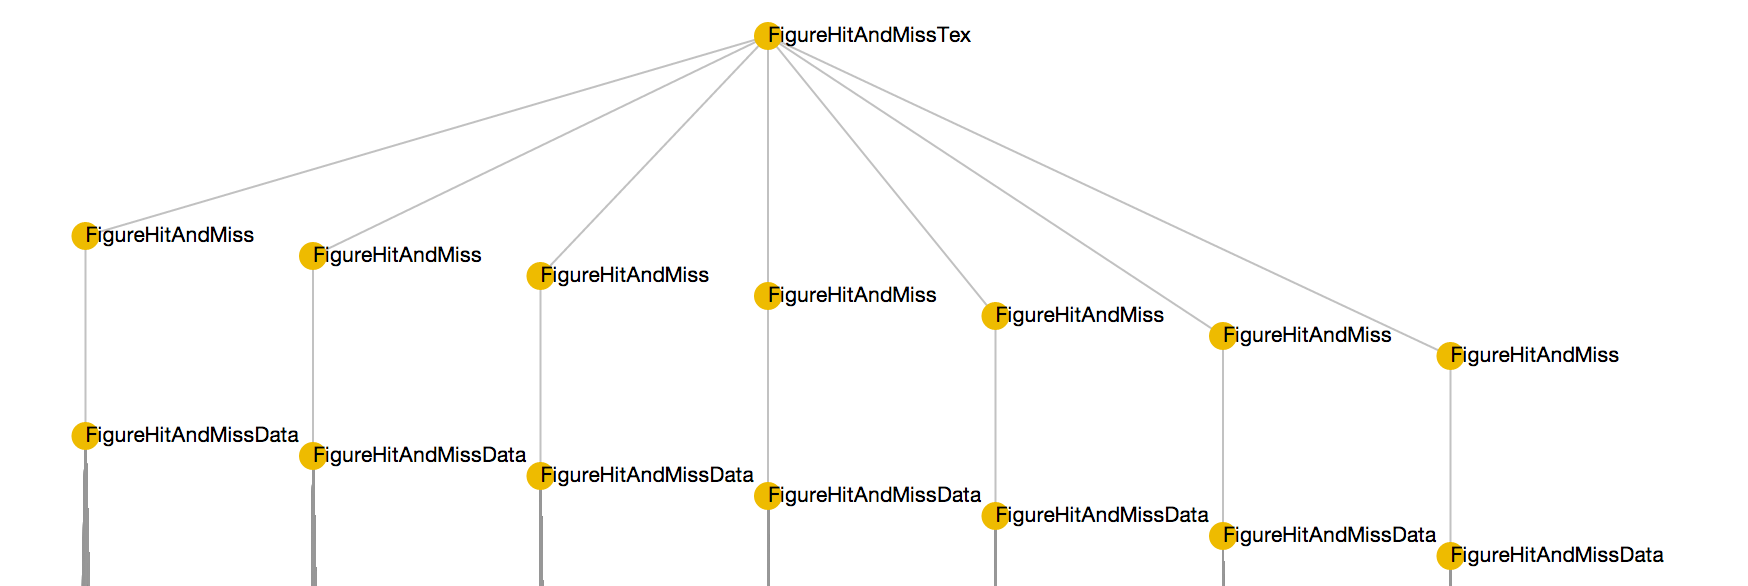
\includegraphics[width=\textwidth]{images/FigureHitAndMissTex.png}
        \caption{Compilation of the {\tt FigureHitAndMissData} tasks into sets of contour plots to be directly embedded to the report.}
        \label{fig:pipes_example:FigureHitAndMissTex}
    \end{subfigure}
    \caption{\emph{Graphical way of describing the dependancies between the tasks used to generate the contour plots of solver performance.} 
    Each  \texttt{TrajectoryTask} depends on \texttt{MEATask} (\ref{fig:pipes_example:TrajectoryTask}).
    A number of these tasks, one for each point of the parameter space, is required to compile the grid of we want to plot as a contour plot.
    Besides the regular trajectories, one trajectory per parameter space obtained using \acrlong{ssa} is also needed (\ref{fig:pipes_example:FigureHitAndMissData}).
    The obtained trajectories can then be used to compute the distance grid, and these grids could be drawn as contour plots and compiled together into \LaTeX{} figures (\ref{fig:pipes_example:FigureHitAndMissTex}).
    Dependancy graphs were drawn by the {\tt luigi} package. }
    \label{fig:pipes_example}
\end{figure}

\autoref{fig:pipes_example} illustrates these concepts by a set of the dependency graphs used to generate the contour plots in \todo{link}.
As mentioned previously, \verb"TrajectoryTask" directly depends on the \verb"MEATask" to provide a set of \glspl{ode} approximating the behaviour of the system. 
This dependancy, is directly pictured in \autoref{fig:pipes_example:TrajectoryTask}. 
We can then use a set of these \verb"TrajectoryTask"s, one for each point on the grid, along with a set of the \verb"SSATrajectoryTask"s, for the same points to compute the numeric grid required to plot the contour. We call this task \verb"FigureHitAndMissData"\footnote{The name \emph{hit-and-miss} comes from the early version of the figure that had only the areas where the solvers failed marked and resembled a dartboard with a couple of darts on it.}, and picture a part of it in \autoref{fig:pipes_example:FigureHitAndMissData}. 
Finally, this data task could be used to produce a contour plot, as ensured by the so-called \verb"FigureHitAndMissTask". 
A set of the contour plots are then fed int o the \verb"FigureHitAndMissTex" task to create a \LaTeX{} figure, much resembling the ones in \todo{cite} (\autoref{fig:pipes_example:FigureHitAndMissTex}).

As one can see from the \autoref{fig:pipes_example}, the hierarchical nature of these dependancies is hard to visualise, let alone to implement efficiently.
Using {\tt luigi} package not only allowed us to skip the implementation step for dependancy management, but also allowed to be more flexible with the figures we are trying to draw -- enabling us to perform large changes to their structure, as we knew that only a small part of the whole system had to be changed at a time.

\subsection{Investigation of MEA and Solver Performance}

Finally, I worked on generalisation of the results obtained by QG in \autoref{GR:sec:results:mea_performance} of the group report. 
I have investigated how the results change depending on the region of parameter space we are, as well as the impact different \gls{ode} solving heuristics have on these results.

Due to the time constraints I have only considered \pft{} model, and \texttt{ode15s}, \texttt{euler}, \texttt{dopri5} and \texttt{rodas} solvers. 
I have found that certain regions of the parameter space are easier to approximate than others, and there exist regions of parameter space that solvers struggle to approximate. These results are discussed in \autoref*{GR:sec:hit-and-miss} of the main report, and I will not reiterate them here to keep this report succinct.

While there were variations in the stability and runtime of the solvers, I have found all of the solvers tested to handle the easy-to-simulate regions well, but fail to produce anything meaningful for the hard ones.
The specific contour plots for the solvers were not included to the main report, but are included in the appendix of this document instead. \todo{link}.



\section{Conclusions}

